\documentclass{BGSU}
% template.tex version 1.3

\title{Dissertation title goes here}
\author{Name of student}
\degree{DOCTOR OF PHILOSOPHY}
\date{June 2015}

\advisor{Name of advisor}
\gfr{\\Name of graduate faculty representative} % graduate faculty representative
\committee{\\Names of other \\committee members}  % put \\ after each name

\usepackage{amsmath}
\usepackage{amssymb}    % allows the use of AMS symbols like blackboard bold
\usepackage{graphicx}
\usepackage{caption}
\usepackage{amsthm}     % allows AMS definitions for theorems, proofs, etc.
\usepackage{epstopdf}
\usepackage{times}    % Times New Roman
\usepackage{titlesec} % allow to change the heading format 
\newtheorem{theorem}{\bf Theorem}[chapter]         % Allow numbered theorems
\newtheorem{proposition}[theorem]{\bf Proposition} % Number props with theorems
\newtheorem{remark}[theorem]{\bf Remark}           % Number remarks too
\newtheorem{lemma}{Lemma}[chapter]
\numberwithin{equation}{chapter}
\setcounter{equation}{0}


% The first level headings need to be centered and 12 point size
\titleformat{\chapter}[display]% NEW
    {\fontsize{12}{15}\bfseries\centering}{\chaptertitlename\ \thechapter}{1em}{}  %\fontsize{<size>}{<line space>}
\titleformat{\section}
    {\fontsize{12}{15}\bfseries}{\thesection}{1em}{}
\titleformat{\subsection}
    {\fontsize{12}{15}\bfseries}{\thesubsection}{1em}{}

\begin{document}

\frontmatter

\maketitle

\copyrightpage

\begin{abstract}

















\end{abstract}

%\mbox{}\newpage\mbox{} % this will give one blank page.
% optional section ``Some students choose to personalize their manuscripts
% with an appropriate quotation or illustration''
% formatting and placement is up to you.

% optional but encouraged section ``as a means to recognize and express
% appreciation to the people who were influential in preparing and completing
% the manuscript''
\begin{acknowledgments}
Text of acknowledgments goes here.





\end{acknowledgments}

\mbox{}\newpage
\tableofcontents

\listoffigures

\mbox{}\newpage\mbox{}  % this will give one blank page.
\listoftables

\mainmatter % starts over page counter and gives regular page numbers

\chapter{Chapter 1 title here}
\numberwithin{equation}{chapter}
\setcounter{equation}{0} \numberwithin{equation}{section}

\section{Thoreau}
You never gain something but that you lose something.\\
		-- Thoreau
\section{Unknown}
And dropping a barbell he points to the sky\\

\begin{figure}[h]
\centering
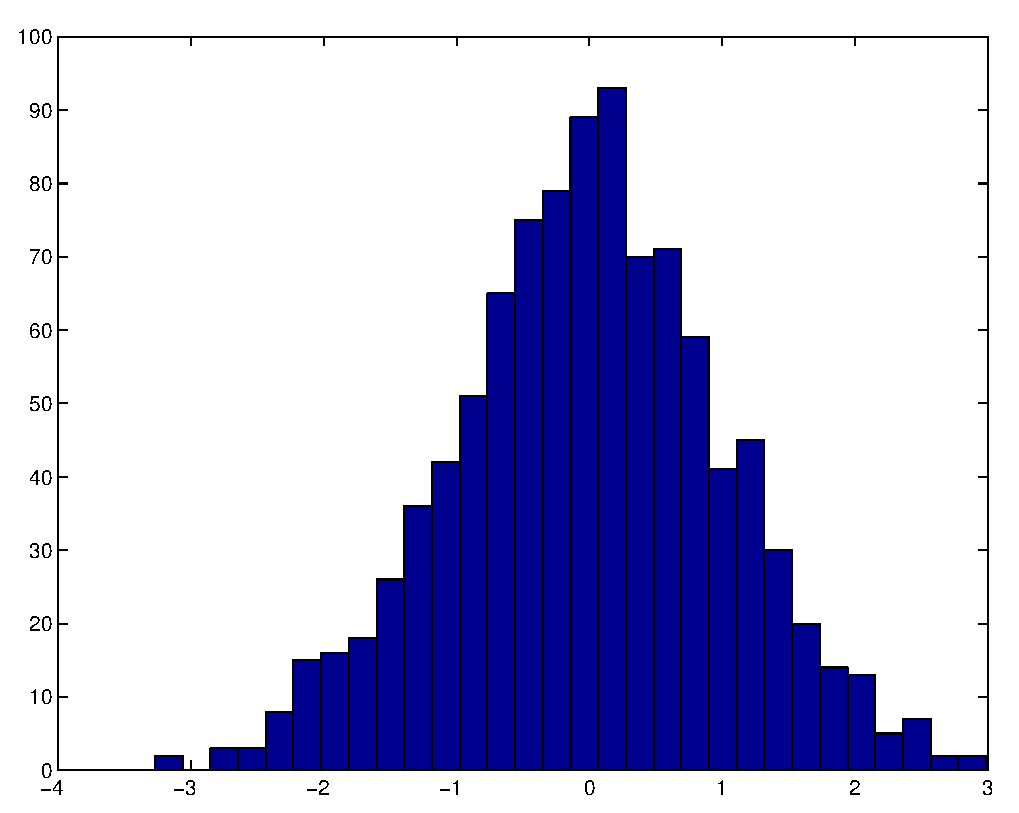
\includegraphics[width = 4.5 in ]{figure.eps}
\caption{Caption of a figure.}\label{FigureLabel}
\end{figure}

\begin{table}[h]
\centering \caption{The values of test
statistics and the corresponding critical values
at~$t_0.$~~$\alpha=0.1.$~}\label{stanford}\vskip .1in
\begin{tabular}{|c|c|c|c|c|c|c|}\hline
$t_0$ & 30 & 60 & 90 & 120 & 150 & 180 \\ \hline
Critical Value & 11.2282 & 10.5357 & 11.1108 & 11.7942 & 11.7343 & 11.7471\\ \hline
Test Statistic & 25.3182 & 24.6395 & 24.6049 & 25.6623 & 27.1320 & 29.3247\\ \hline
\end{tabular}
\end{table}

\section{Citations}

%If you use the package natbib for citations, here is the example how to cite an article.
%Many thanks to Dr. Maria Rizzo who worked this section.

To cite an article use cite, citet, or citep.

For ``in text'' citations use citet:  The original result is attributed to \citet{vn28}.
Refer to \citet{mardia70} for an example.
Refer to \cite{mardia70} for an example.

For a ``parenthetical citation'' use citep:  The computations were implemented in R \citep{R}
using bootstrap \citep{dh97,et93}.

When citing a book, it is helpful to mention where to find the result by indicating
a chapter or a page number or an equation number:  \citet[Ch.~6]{et93} discuss additional results.

Add your reference information to the file reference.bib.
Every time you edit reference.bib, run BibTeX on the dissertation.tex file so that LaTeX will know what the references are.

%If you don't want to use natbib, you should insert comment (\%) in the above part.  
%Here is the example to cite an article without using natbib package. \cite{forina1991class}


\begin{sidewaysfigure}[p!]
\centering
{bf Landscape figure}
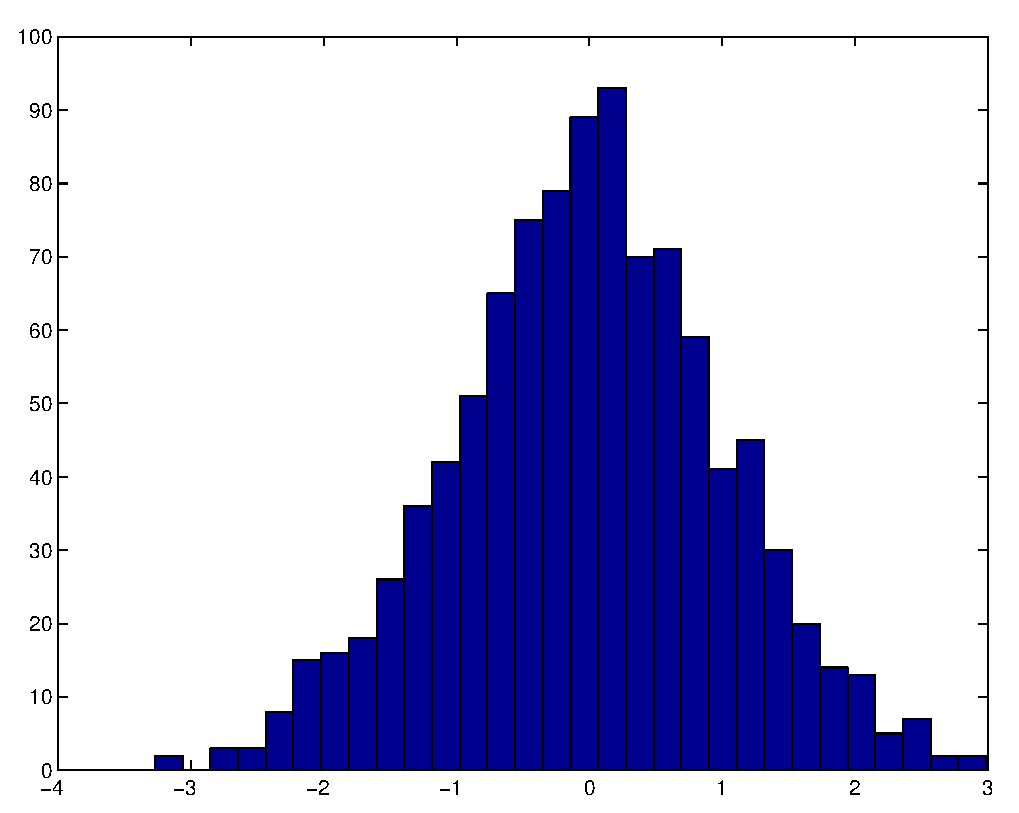
\includegraphics[width=\hsize-1in]{figure.eps}
\caption[Short label for List of Figures]{ 
Long label for under the actual figure.}
\end{sidewaysfigure}



\begin{landscape}
\thispagestyle{lscape}
\pagestyle{lscape}
  \begin{figure}
    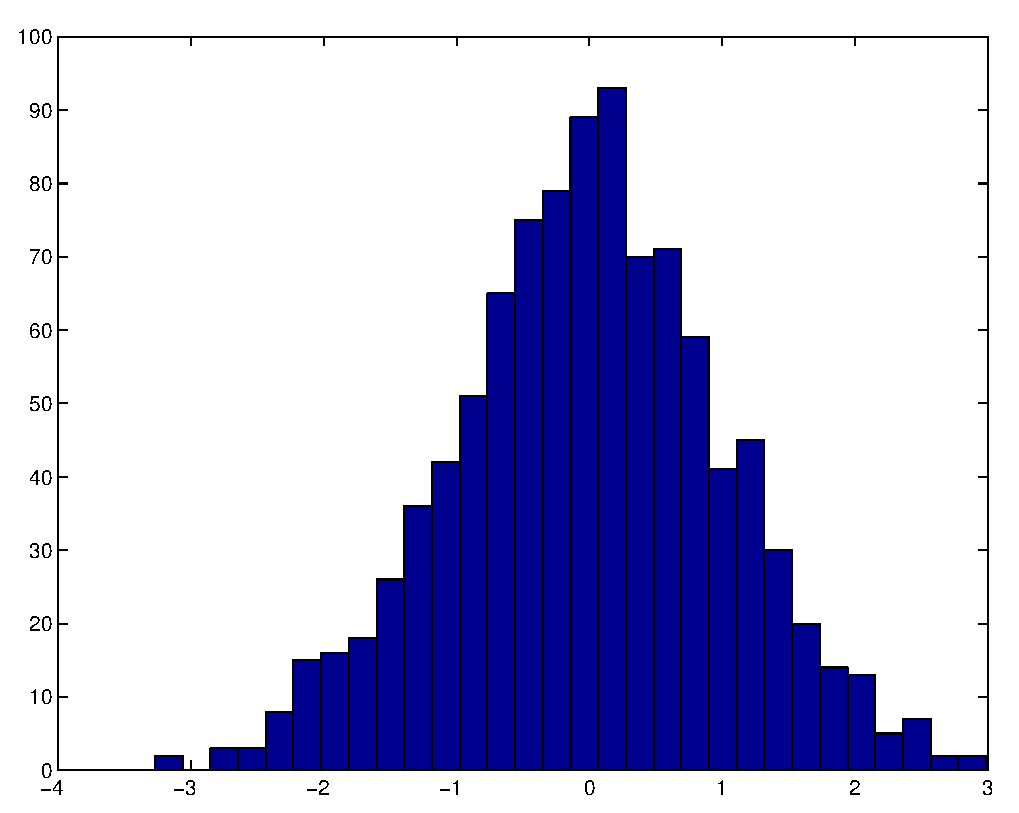
\includegraphics[width=\linewidth,height=\textheight-1in]{figure.eps}
    \caption[Short caption for List of Figures]{Long caption to appear under the figure.  Hopefully the figure is not so large that there is no room for the caption, because then the caption might move to a different page, or the text might go into the margin, and that would be bad!}
  \end{figure}
\end{landscape}


%\mbox{}\newpage\mbox{}
\chapter{Chapter 2 title here}
\numberwithin{equation}{chapter}
\setcounter{equation}{0} \numberwithin{equation}{section} 

John the Baptist after poisoning a thief,
Looks up at his hero, the Commander-in-Chief,
Saying tell me great leader, but please make it brief
Is there a hole for me to get sick in?
 The Commander-in-Chief answers him while chasing a fly,
Saying death to all those who would whimper and cry.
And dropping a barbell he points to the sky,
Saying the sun is not yellow, it's chicken.
		-- Bob Dylan, "Tombstone Blues"



%\mbox{}\newpage\mbox{}
\chapter{Chapter 3 title here}
\numberwithin{equation}{chapter}
\setcounter{equation}{0} \numberwithin{equation}{section}

%\mbox{}\newpage\mbox{}
\chapter{Chapter 4 title here}
\numberwithin{equation}{chapter}
\chapter{\texorpdfstring{HOW TO PROVE IT}{}} %upper case only
\setcounter{equation}{0} 
\numberwithin{equation}{section}

\section{proof by accumulated evidence:}

	Long and diligent search has not revealed a counterexample.

\section{proof by cosmology:}

	The negation of the proposition is unimaginable or
	meaningless. Popular for proofs of the existence of God.

\section{proof by mutual reference:}

	In reference A, Theorem 5 is said to follow from Theorem 3 in
	reference B, which is shown to follow from Corollary 6.2 in
	reference C, which is an easy consequence of Theorem 5 in
	reference A.

\section{proof by metaproof:}

	A method is given to construct the desired proof. The
	correctness of the method is proved by any of these
	techniques.


%\mbox{}\newpage\mbox{}
\chapter{Chapter 5 title here}
\numberwithin{equation}{chapter}
\chapter{\texorpdfstring{OTHERNESS}{}} %upper case only
\setcounter{equation}{0} 
\numberwithin{equation}{section}

In a surprise raid last night, federal agents ransacked a house in search
of a rebel computer hacker.  However, they were unable to complete the arrest
because the warrant was made out in the name of Don Provan, while the only
person in the house was named don provan.  Proving, once again, that Unix is
superior to Tops10.

\section{deja-vu}

Over the years, I've developed my sense of deja vu so acutely that now
I can remember things that *have* happened before ...

\section{More references}

Once again, we can refer back to Equation \ref{PythagoreanTheorem}.
We can also refer to Equation \ref{squarebinomial}.
Finally, we can refer back to Section \ref{AdditionalNumberedResults}.








\backmatter


\mbox{}\newpage\mbox{}
% for using bibtex (you may use other bibliography types)
\begin{thebibliography}{99}

\bibitem{} Alam, K. and Cahoy, D.O. (1999). A test for equality of
variances. \textit{Journal of Mathematical Sciences, Philippines,} {\bf{2}}(1), 1-19.

\end{thebibliography}
\mbox{}\newpage
\phantomsection
\appendix
\chapter{Appendix: Title of appendix}
\chapter{\texorpdfstring{APPENDIX A\hspace{1em}SELECTED R PROGRAMS}{APPENDIX A}}

Text of appendix goes here.

% If you want to put program codes in the appendix, here is one example. 
\begin{itemize}
\item The function kernel is used to compute the kernel function of variances
{\small
\begin{lstlisting}
kernel<-function(x,y){
  h <- 0.5*(x-y)^2
  return(h)
}
\end{lstlisting}
}
\end{itemize}


\end{document}
